\subsection{Perfil dos Dados (Data Profiling)}
\label{subsec:data_profiling}

O \textit{Data Profiling} constitui uma etapa fundamental na análise exploratória, permitindo aferir a estrutura, qualidade e integridade dos dados antes da sua integração no \textit{Data Warehouse}. Esta secção detalha a análise efetuada sobre o conjunto de dados principal, proveniente do Instituto da Conservação da Natureza e das Florestas (ICNF).

A análise incidiu sobre 23 variáveis selecionadas pela sua relevância para os objetivos do projeto, abrangendo dimensões geográficas, temporais, métricas de severidade e contexto meteorológico. Dado que as restantes fontes de dados (ex: Open-Meteo) foram integradas por derivação espacial e temporal a partir deste \textit{dataset} base, a validação da qualidade dos dados do ICNF assume um papel central na fiabilidade do sistema.

\subsubsection{Análise de Completude}
A verificação de valores nulos evidenciou padrões distintos de preenchimento. Destaca-se a elevada taxa de ausência nas variáveis meteorológicas originais, reflexo de limitações na cobertura histórica da rede de estações ou falhas no registo sistemático.

A ausência de dados em cerca de 30\% dos registos climáticos (Tabela \ref{tab:nulls}) reforçou a decisão de ignorar estes campos em favor da integração com a API do \textit{Open-Meteo}. Esta abordagem garante não só a completude total das variáveis climáticas, como também o acesso a um leque mais alargado de indicadores atmosféricos.

Por outro lado, as variáveis categóricas de classificação (TIPO, CAUSA, TIPOCAUSA) apresentam uma elevada completude (superior a 93\%). Contudo, apesar da baixa incidência de nulos nas variáveis da família "Causa" e nos índices de perigo (FFMC e FWI), optou-se por isolar os registos incompletos em tabelas de quarentena. Esta estratégia permite uma validação posterior sem comprometer a carga dos dados válidos, salvaguardando variáveis cruciais para a análise de risco.

\begin{table}[htbp]
	\centering
	\caption{Análise de valores nulos por variável}
	\label{tab:nulls}
	\begin{tabular}{lccc}
		\hline
		\textbf{Variável} & \textbf{Nulos (\%)} & \textbf{Nulos (Qtd)} & \textbf{Total Registos} \\
		\hline
		TEMPERATURA & 29.9 & 732 & 2451 \\
		HUMIDADERELATIVA & 29.9 & 732 & 2451 \\
		CAUSA & 7.5 & 184 & 2451 \\
		TIPOCAUSA & 7.5 & 184 & 2451 \\
		CAUSAFAMILIA & 7.5 & 184 & 2451 \\
		FFMC & 0.2 & 6 & 2451 \\
		FWI & 0.2 & 6 & 2451 \\
		\hline
	\end{tabular}
\end{table}

\subsubsection{Unicidade e Duplicados}
A integridade referencial e a unicidade dos registos são pré-requisitos essenciais para evitar a distorção de medidas agregadas no \textit{Data Warehouse}.

A análise confirmou a inexistência de identificadores (\textit{IDs}) duplicados ou de registos inteiramente redundantes. Este resultado valida a qualidade dos dados de origem, dispensando, deste modo, etapas complexas de deduplicação durante o processo de ETL e garantindo que cada ocorrência de incêndio é contabilizada uma única vez nas análises estatísticas.

\subsubsection{Deteção de Outliers}
A análise de distribuição, representada pelos boxplots na Figura \ref{fig:boxplot_individuais}, permitiu identificar o comportamento das variáveis numéricas:

\begin{figure}[htbp]
	\centering
	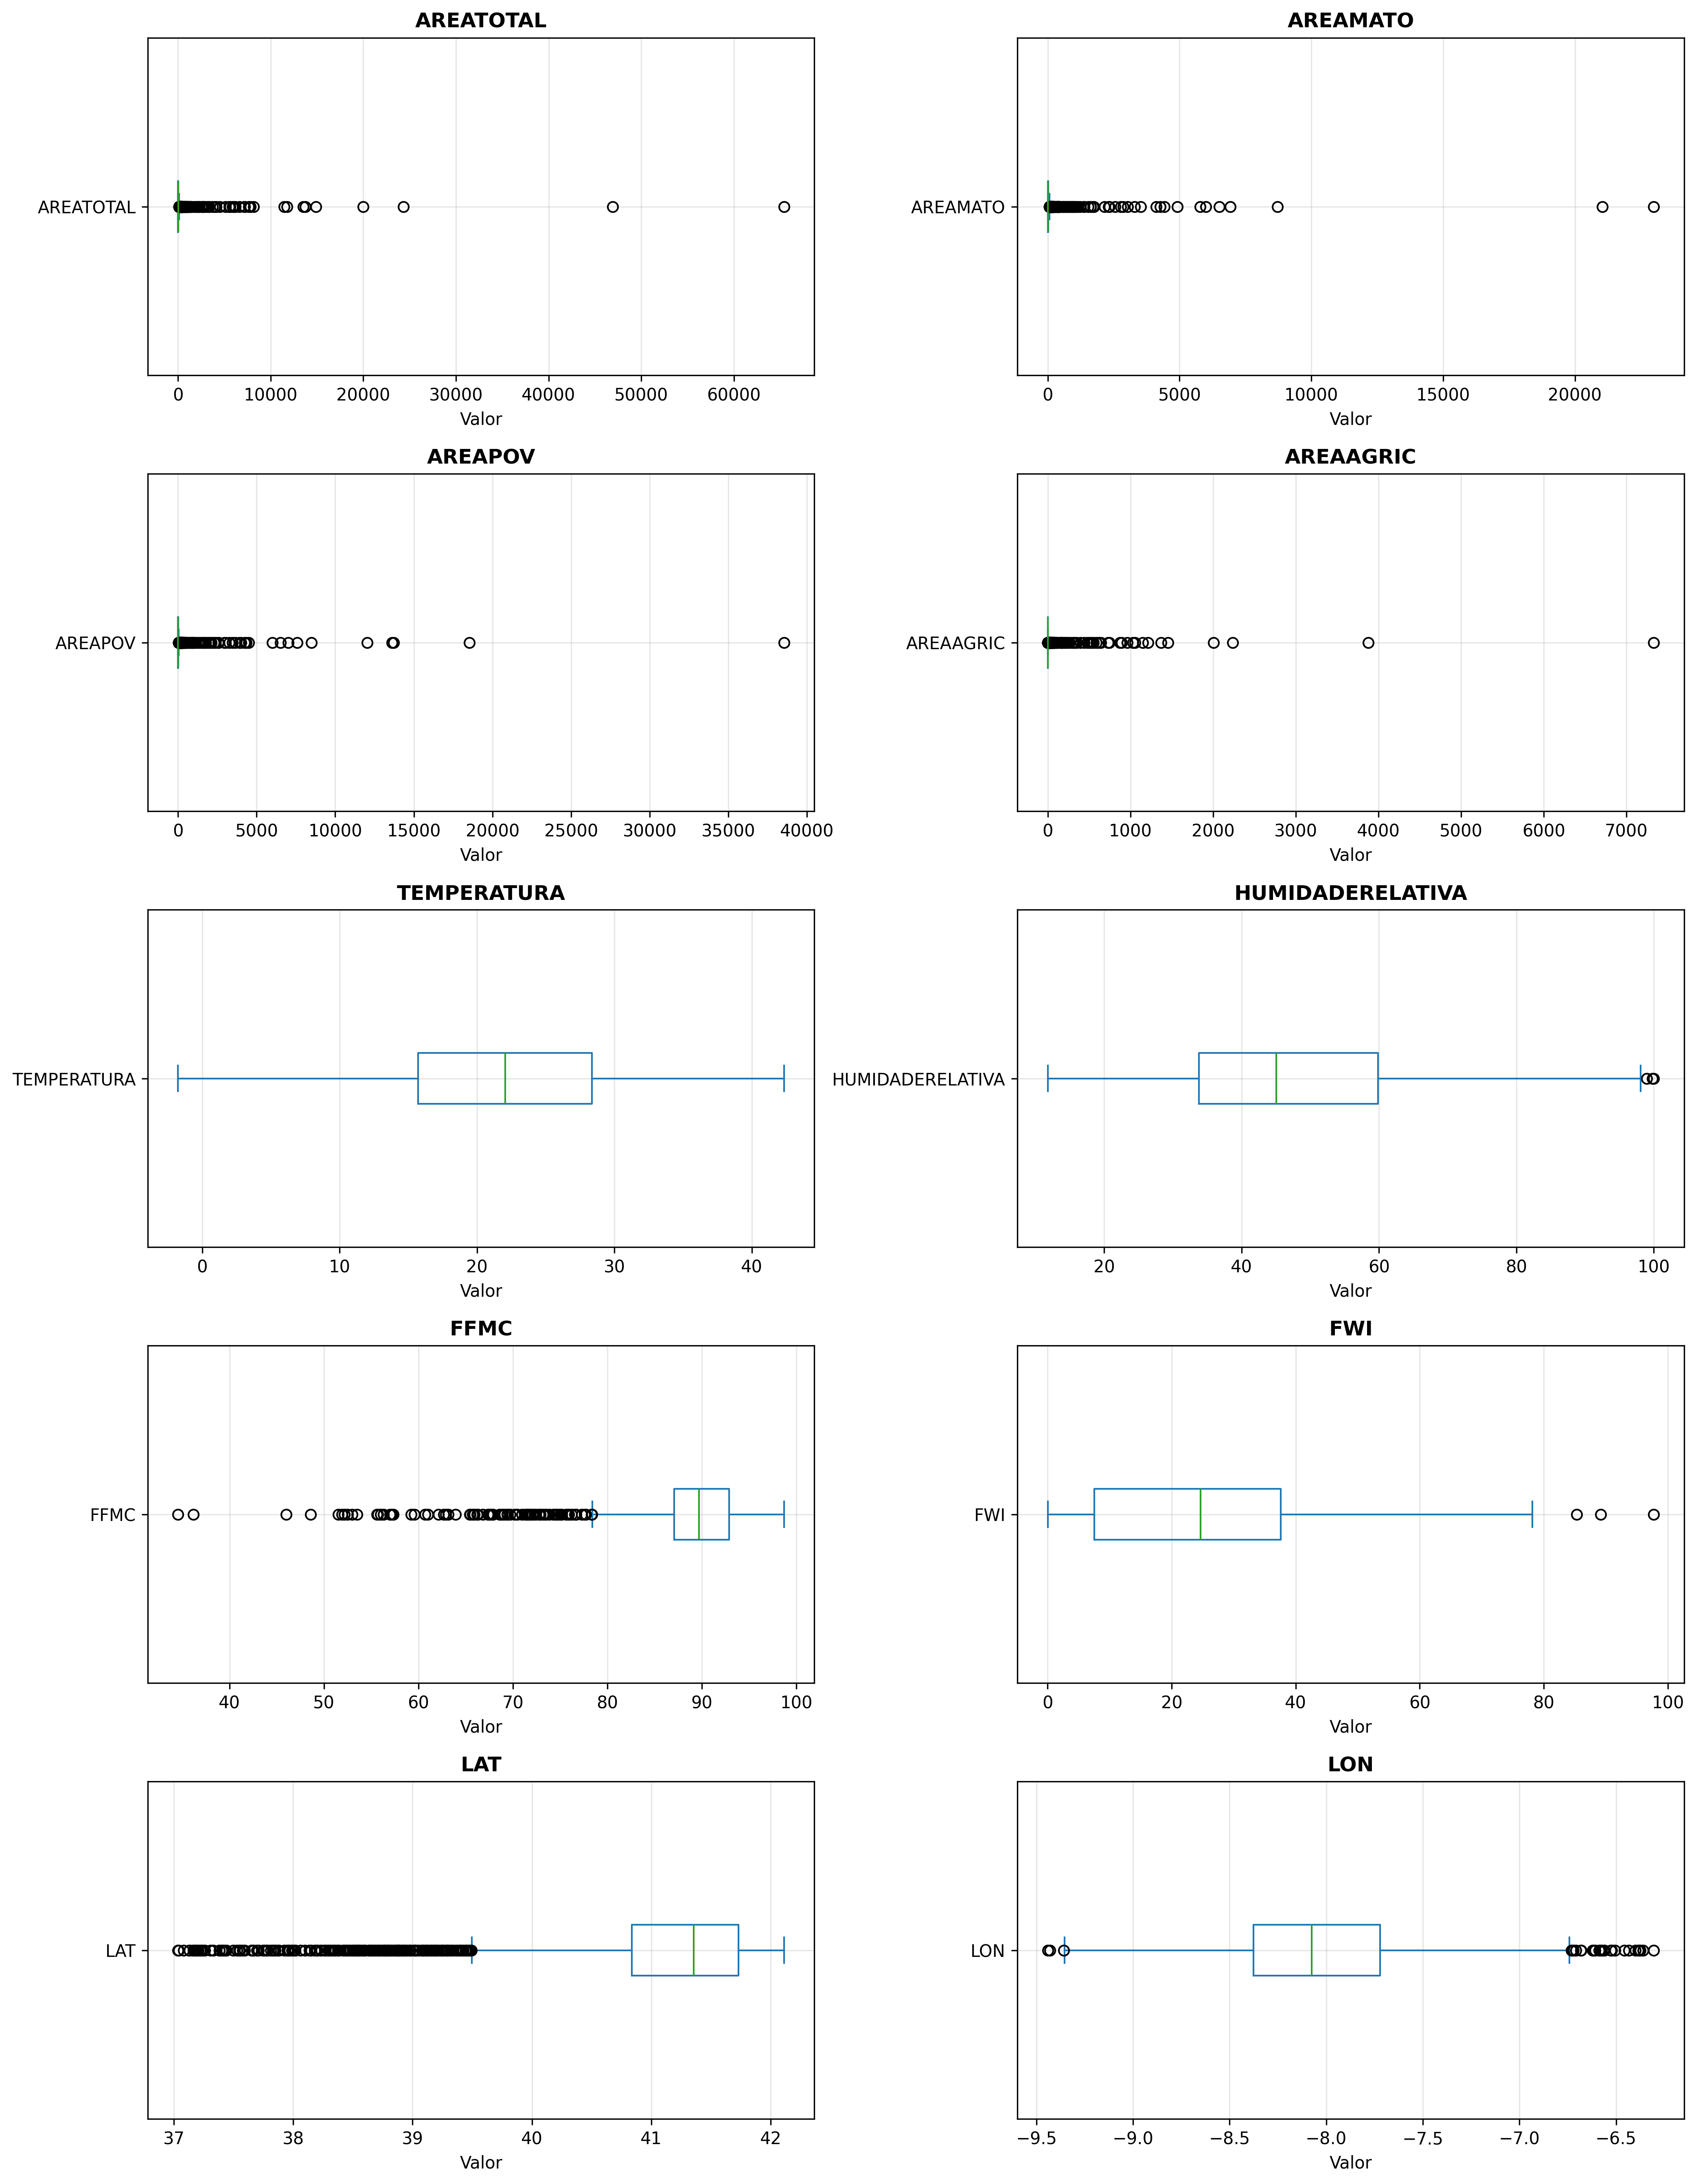
\includegraphics[width=0.8\linewidth]{imagens/07_boxplots_individuais.png}
	\caption{Boxplots das variáveis numéricas do ICNF}
	\label{fig:boxplot_individuais}
\end{figure}

\begin{itemize}
	\item \textbf{Área Ardida:} As variáveis de área (Total, Mato, Povoamento) exibem uma forte assimetria positiva. A concentração de dados em valores baixos, acompanhada por uma longa cauda de \textit{outliers} superiores, é característica do fenómeno dos incêndios florestais: eventos raros, mas de dimensão catastrófica. Estes valores extremos representam ocorrências reais e devem ser preservados.
	\item \textbf{Meteorologia:} A Temperatura segue uma distribuição tendencialmente simétrica, enquanto a Humidade Relativa apresenta \textit{outliers} inferiores consistentes com períodos de seca extrema.
	\item \textbf{Índices de Perigo:} O FFMC e o FWI apresentam \textit{outliers} superiores que sinalizam condições excecionais de perigo de incêndio, validando a sua utilidade como indicadores de alerta.
\end{itemize}

\subsubsection{Distribuição Espacial e Consistência}
A análise geográfica (Figura \ref{fig:20Distritos}) evidencia uma forte concentração de ocorrências nos distritos do interior Norte e Centro. Esta assimetria reflete a interação entre coberto florestal, relevo regional e fatores socioeconómicos.

\begin{figure}[htbp]
	\centering
	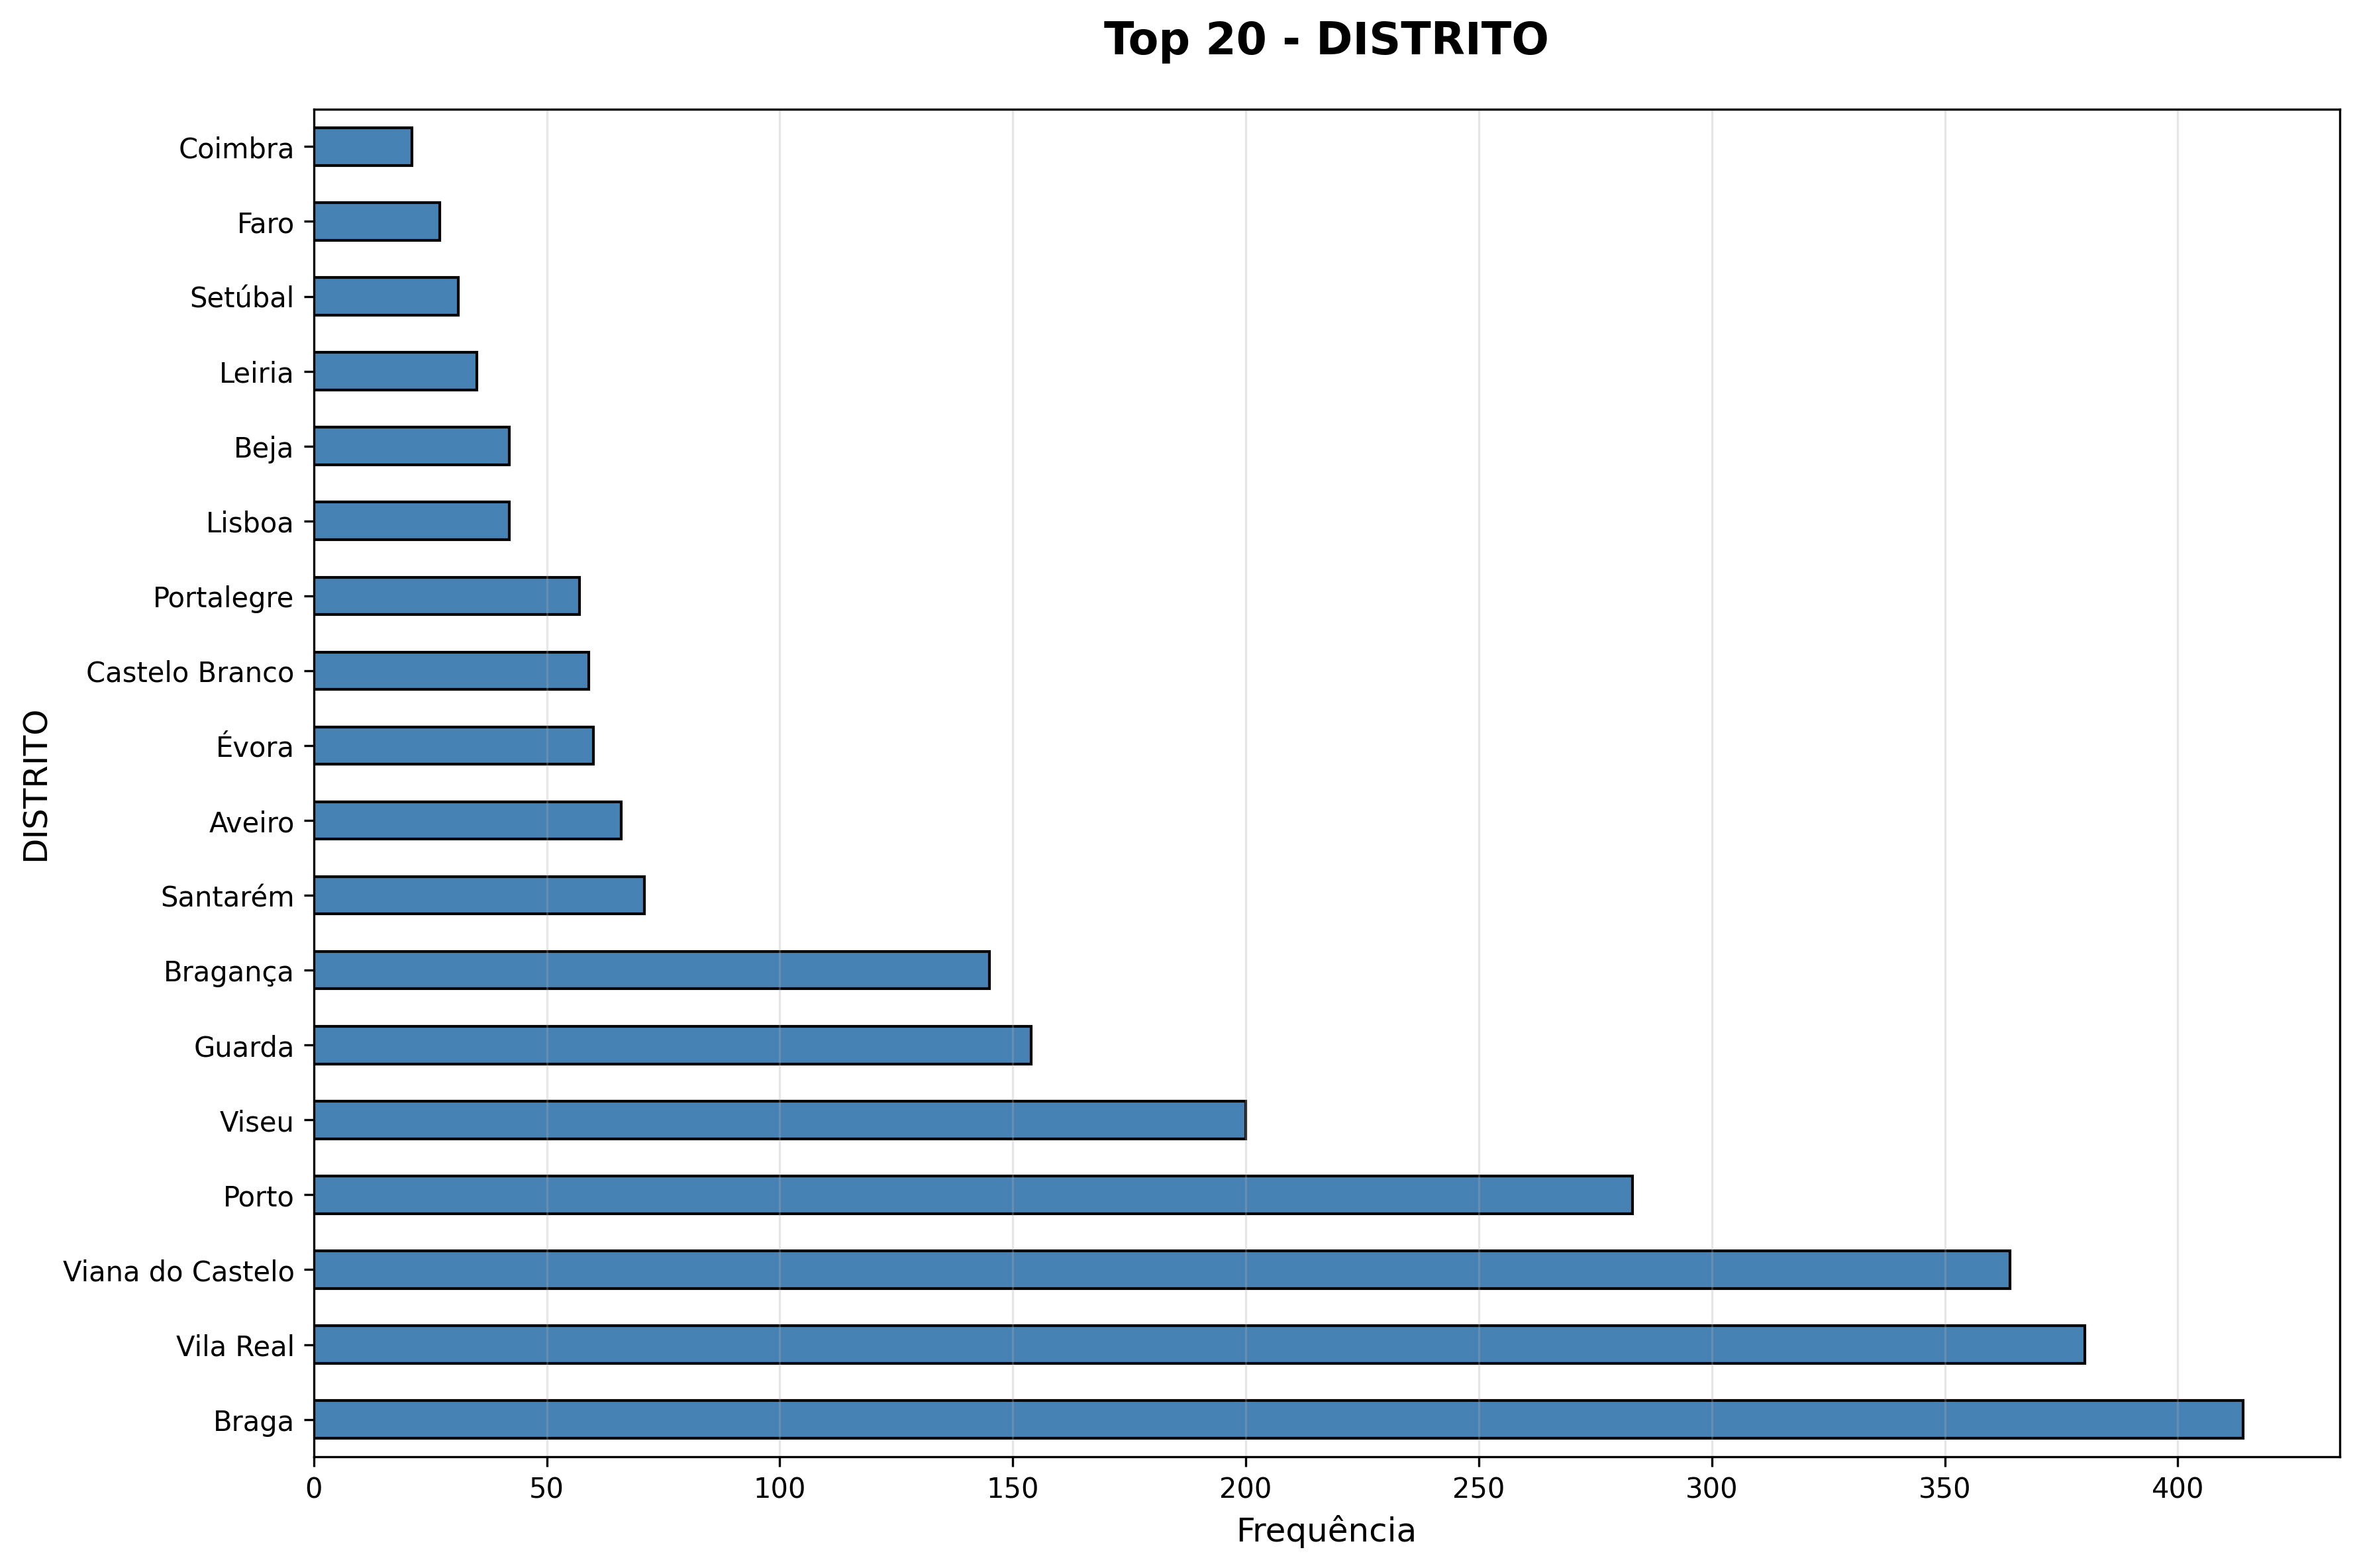
\includegraphics[width=0.8\linewidth]{imagens/03_grafico_DISTRITO.png}
	\caption{Os 20 distritos com maior frequência de ocorrências}
	\label{fig:20Distritos}
\end{figure}

Ao nível da freguesia (Figura \ref{fig:20Freguesias}), identificam-se \textit{hotspots} locais onde a recorrência é crítica. É importante destacar que as freguesias com maior frequência de ignições não correspondem necessariamente às áreas de maior área ardida, sugerindo dinâmicas distintas entre a ocorrência e a propagação do fogo.

\begin{figure}[htbp]
	\centering
	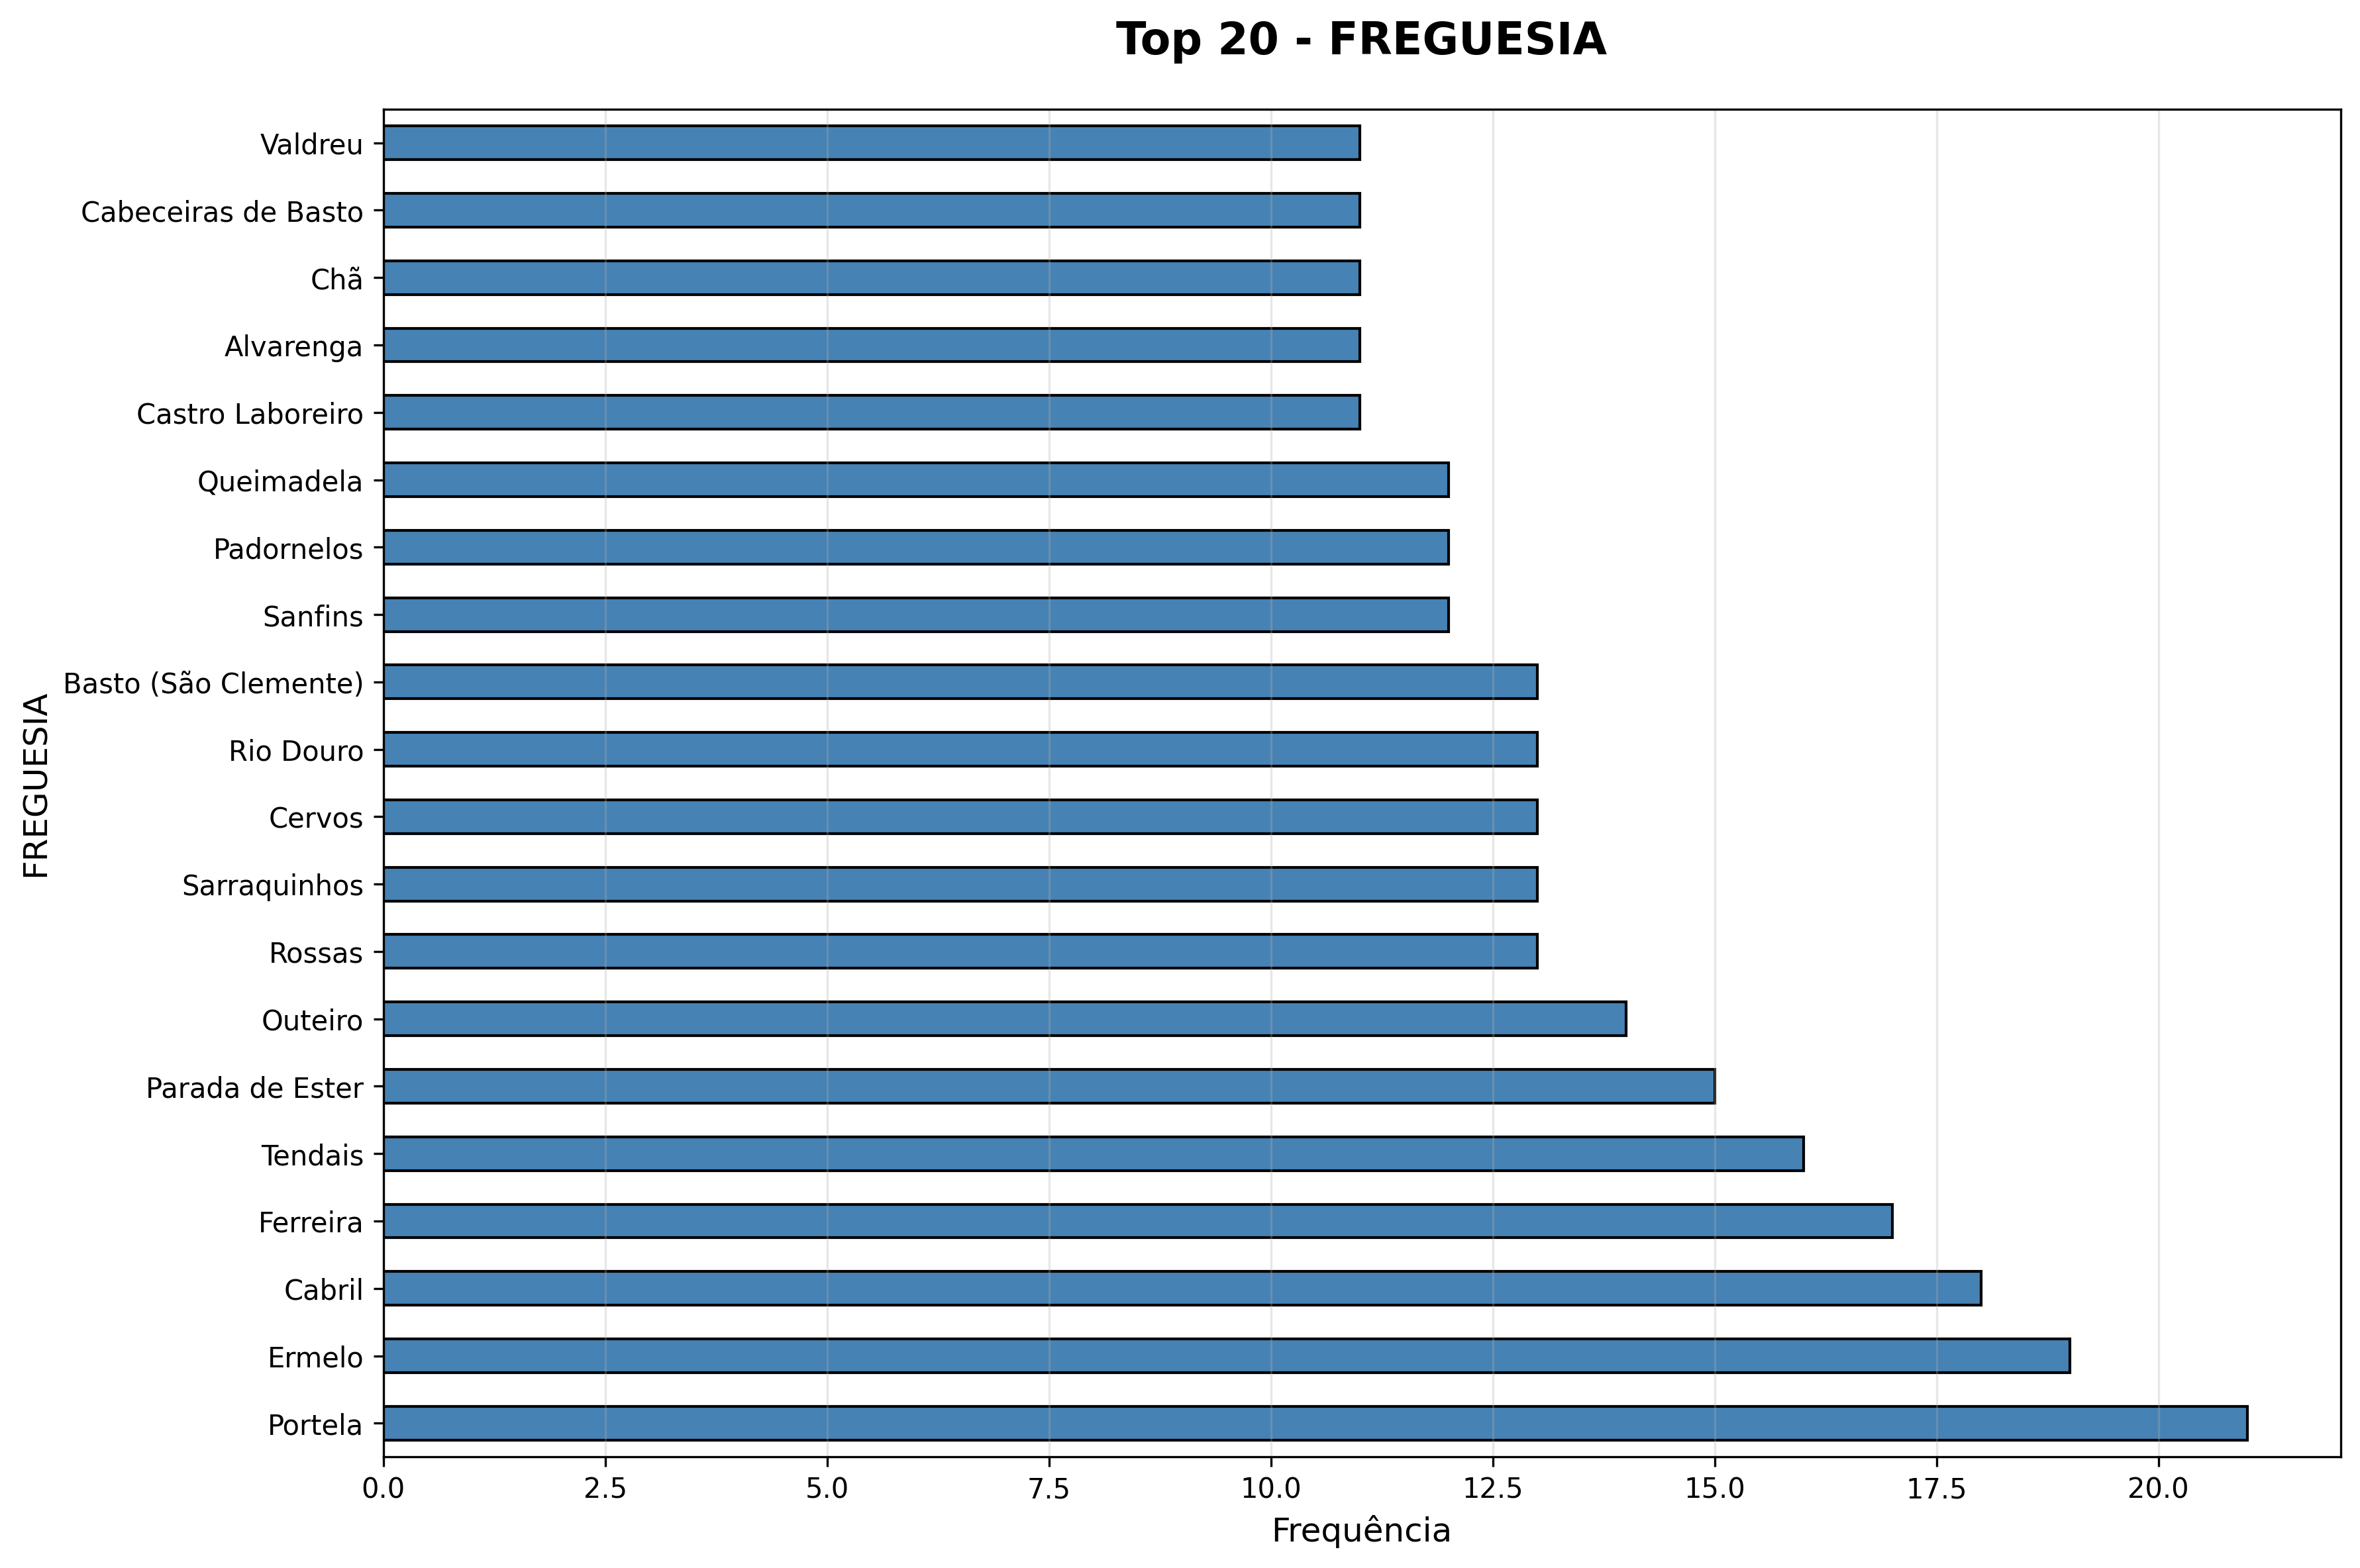
\includegraphics[width=0.8\linewidth]{imagens/03_grafico_FREGUESIA.png}
	\caption{As 20 freguesias com maior frequência de ocorrências}
	\label{fig:20Freguesias}
\end{figure}

Relativamente à qualidade dos dados categóricos, salienta-se que a geração destes gráficos não exigiu qualquer normalização prévia de texto. A ausência de categorias duplicadas por erros de sintaxe (ex: "Aveiro" vs "aveiro ") demonstra a consistência das dimensões geográficas na fonte, simplificando a criação de tabelas de dimensão.

\subsubsection{Análise Causal e Correlações}
A matriz de correlações (Figura \ref{fig:correlacoes}) permitiu validar relações esperadas e identificar variáveis redundantes para a modelação dimensional.

\begin{figure}[htbp]
	\centering
	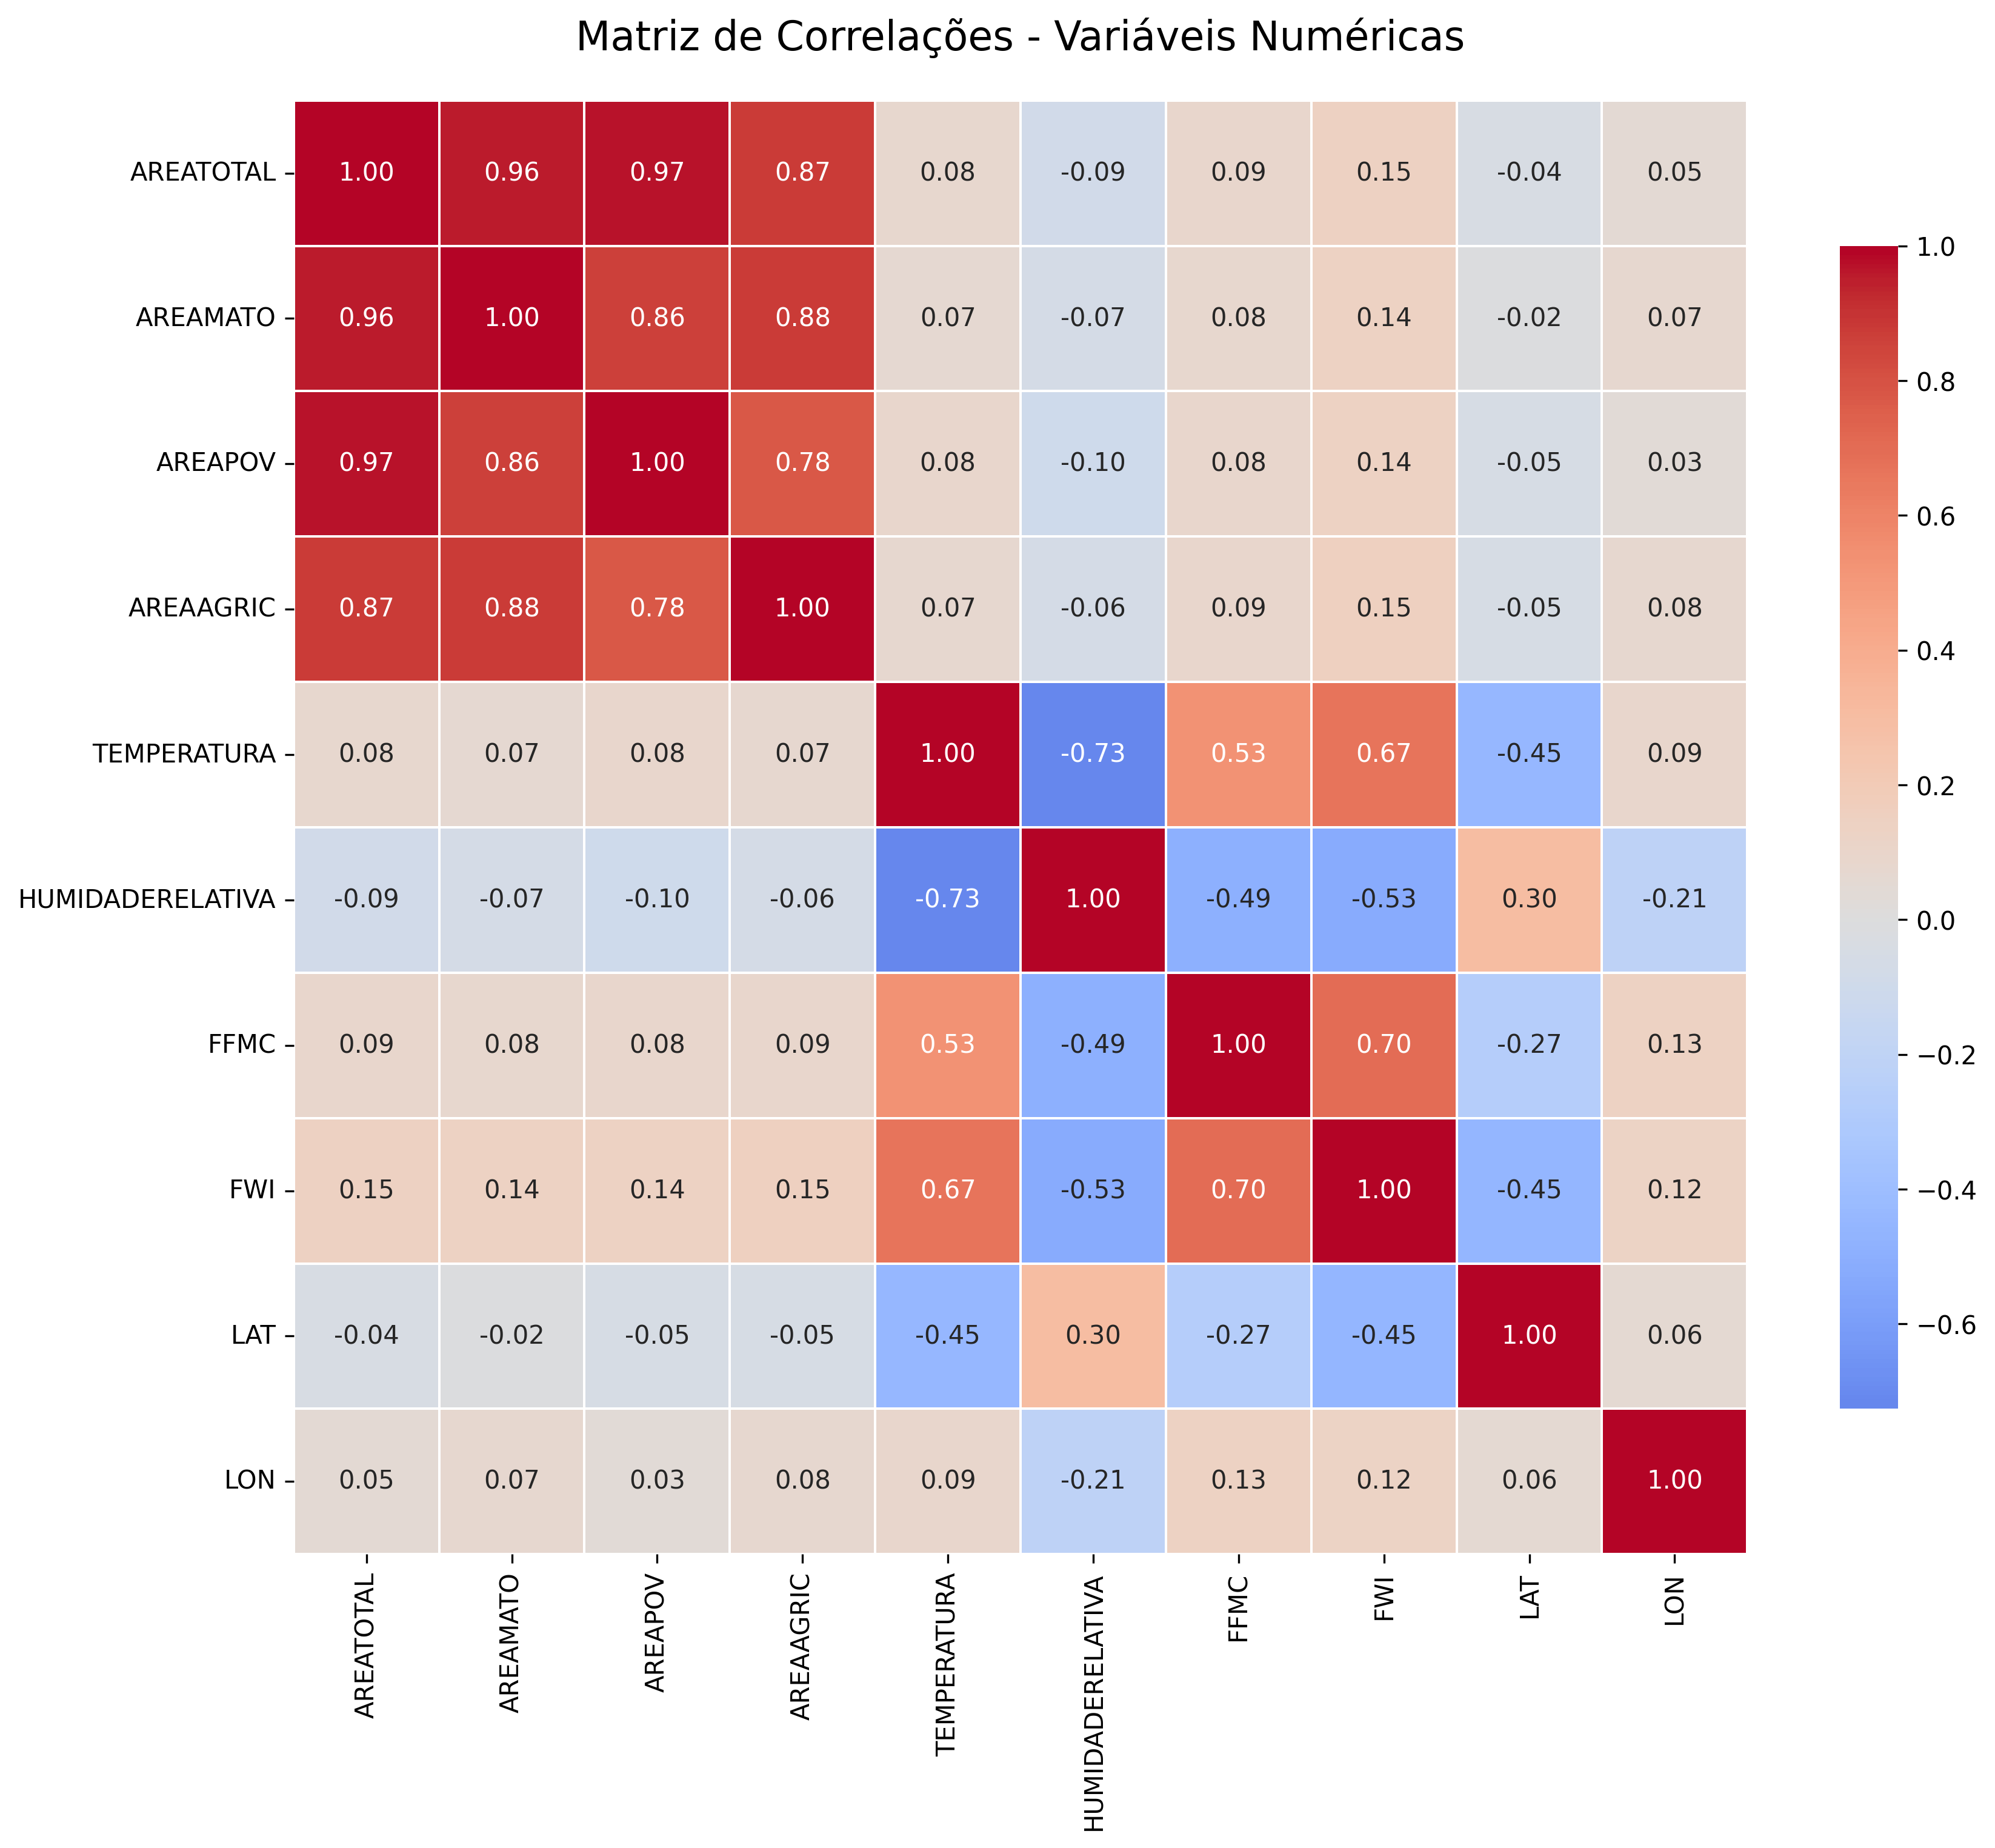
\includegraphics[width=0.7\linewidth]{imagens/06_correlacoes.png}
	\caption{Matriz de correlações (Pearson) entre variáveis numéricas}
	\label{fig:correlacoes}
\end{figure}

Da análise destacam-se as seguintes relações lineares:
\begin{itemize}
	\item \textbf{Composição da Área Ardida:} Correlações fortes ($r > 0.7$) entre a Área Total e as suas componentes (Mato/Povoamento), indicando a predominância do tipo de vegetação afetado.
	\item \textbf{Fatores Meteorológicos:} A correlação negativa entre Temperatura e Humidade Relativa, bem como a forte correlação entre os índices FFMC e FWI, validam a consistência física dos dados.
	\item \textbf{Severidade vs. Clima:} As correlações moderadas entre índices meteorológicos e área ardida sugerem que, embora o clima propicie as condições para grandes incêndios, a dimensão final da ocorrência depende de outros fatores operacionais (meios de combate, acessibilidades), justificando a inclusão destas variáveis no modelo multidimensional.
\end{itemize}